% Options for packages loaded elsewhere
\PassOptionsToPackage{unicode}{hyperref}
\PassOptionsToPackage{hyphens}{url}
\PassOptionsToPackage{dvipsnames,svgnames,x11names}{xcolor}
%
\documentclass[
  12pt,
  letterpaper,
  DIV=11,
  numbers=noendperiod]{scrartcl}

\usepackage{amsmath,amssymb}
\usepackage{lmodern}
\usepackage{iftex}
\ifPDFTeX
  \usepackage[T1]{fontenc}
  \usepackage[utf8]{inputenc}
  \usepackage{textcomp} % provide euro and other symbols
\else % if luatex or xetex
  \usepackage{unicode-math}
  \defaultfontfeatures{Scale=MatchLowercase}
  \defaultfontfeatures[\rmfamily]{Ligatures=TeX,Scale=1}
\fi
% Use upquote if available, for straight quotes in verbatim environments
\IfFileExists{upquote.sty}{\usepackage{upquote}}{}
\IfFileExists{microtype.sty}{% use microtype if available
  \usepackage[]{microtype}
  \UseMicrotypeSet[protrusion]{basicmath} % disable protrusion for tt fonts
}{}
\makeatletter
\@ifundefined{KOMAClassName}{% if non-KOMA class
  \IfFileExists{parskip.sty}{%
    \usepackage{parskip}
  }{% else
    \setlength{\parindent}{0pt}
    \setlength{\parskip}{6pt plus 2pt minus 1pt}}
}{% if KOMA class
  \KOMAoptions{parskip=half}}
\makeatother
\usepackage{xcolor}
\usepackage[margin=1in]{geometry}
\setlength{\emergencystretch}{3em} % prevent overfull lines
\setcounter{secnumdepth}{-\maxdimen} % remove section numbering
% Make \paragraph and \subparagraph free-standing
\ifx\paragraph\undefined\else
  \let\oldparagraph\paragraph
  \renewcommand{\paragraph}[1]{\oldparagraph{#1}\mbox{}}
\fi
\ifx\subparagraph\undefined\else
  \let\oldsubparagraph\subparagraph
  \renewcommand{\subparagraph}[1]{\oldsubparagraph{#1}\mbox{}}
\fi

\usepackage{color}
\usepackage{fancyvrb}
\newcommand{\VerbBar}{|}
\newcommand{\VERB}{\Verb[commandchars=\\\{\}]}
\DefineVerbatimEnvironment{Highlighting}{Verbatim}{commandchars=\\\{\}}
% Add ',fontsize=\small' for more characters per line
\usepackage{framed}
\definecolor{shadecolor}{RGB}{241,243,245}
\newenvironment{Shaded}{\begin{snugshade}}{\end{snugshade}}
\newcommand{\AlertTok}[1]{\textcolor[rgb]{0.68,0.00,0.00}{#1}}
\newcommand{\AnnotationTok}[1]{\textcolor[rgb]{0.37,0.37,0.37}{#1}}
\newcommand{\AttributeTok}[1]{\textcolor[rgb]{0.40,0.45,0.13}{#1}}
\newcommand{\BaseNTok}[1]{\textcolor[rgb]{0.68,0.00,0.00}{#1}}
\newcommand{\BuiltInTok}[1]{\textcolor[rgb]{0.00,0.23,0.31}{#1}}
\newcommand{\CharTok}[1]{\textcolor[rgb]{0.13,0.47,0.30}{#1}}
\newcommand{\CommentTok}[1]{\textcolor[rgb]{0.37,0.37,0.37}{#1}}
\newcommand{\CommentVarTok}[1]{\textcolor[rgb]{0.37,0.37,0.37}{\textit{#1}}}
\newcommand{\ConstantTok}[1]{\textcolor[rgb]{0.56,0.35,0.01}{#1}}
\newcommand{\ControlFlowTok}[1]{\textcolor[rgb]{0.00,0.23,0.31}{#1}}
\newcommand{\DataTypeTok}[1]{\textcolor[rgb]{0.68,0.00,0.00}{#1}}
\newcommand{\DecValTok}[1]{\textcolor[rgb]{0.68,0.00,0.00}{#1}}
\newcommand{\DocumentationTok}[1]{\textcolor[rgb]{0.37,0.37,0.37}{\textit{#1}}}
\newcommand{\ErrorTok}[1]{\textcolor[rgb]{0.68,0.00,0.00}{#1}}
\newcommand{\ExtensionTok}[1]{\textcolor[rgb]{0.00,0.23,0.31}{#1}}
\newcommand{\FloatTok}[1]{\textcolor[rgb]{0.68,0.00,0.00}{#1}}
\newcommand{\FunctionTok}[1]{\textcolor[rgb]{0.28,0.35,0.67}{#1}}
\newcommand{\ImportTok}[1]{\textcolor[rgb]{0.00,0.46,0.62}{#1}}
\newcommand{\InformationTok}[1]{\textcolor[rgb]{0.37,0.37,0.37}{#1}}
\newcommand{\KeywordTok}[1]{\textcolor[rgb]{0.00,0.23,0.31}{#1}}
\newcommand{\NormalTok}[1]{\textcolor[rgb]{0.00,0.23,0.31}{#1}}
\newcommand{\OperatorTok}[1]{\textcolor[rgb]{0.37,0.37,0.37}{#1}}
\newcommand{\OtherTok}[1]{\textcolor[rgb]{0.00,0.23,0.31}{#1}}
\newcommand{\PreprocessorTok}[1]{\textcolor[rgb]{0.68,0.00,0.00}{#1}}
\newcommand{\RegionMarkerTok}[1]{\textcolor[rgb]{0.00,0.23,0.31}{#1}}
\newcommand{\SpecialCharTok}[1]{\textcolor[rgb]{0.37,0.37,0.37}{#1}}
\newcommand{\SpecialStringTok}[1]{\textcolor[rgb]{0.13,0.47,0.30}{#1}}
\newcommand{\StringTok}[1]{\textcolor[rgb]{0.13,0.47,0.30}{#1}}
\newcommand{\VariableTok}[1]{\textcolor[rgb]{0.07,0.07,0.07}{#1}}
\newcommand{\VerbatimStringTok}[1]{\textcolor[rgb]{0.13,0.47,0.30}{#1}}
\newcommand{\WarningTok}[1]{\textcolor[rgb]{0.37,0.37,0.37}{\textit{#1}}}

\providecommand{\tightlist}{%
  \setlength{\itemsep}{0pt}\setlength{\parskip}{0pt}}\usepackage{longtable,booktabs,array}
\usepackage{calc} % for calculating minipage widths
% Correct order of tables after \paragraph or \subparagraph
\usepackage{etoolbox}
\makeatletter
\patchcmd\longtable{\par}{\if@noskipsec\mbox{}\fi\par}{}{}
\makeatother
% Allow footnotes in longtable head/foot
\IfFileExists{footnotehyper.sty}{\usepackage{footnotehyper}}{\usepackage{footnote}}
\makesavenoteenv{longtable}
\usepackage{graphicx}
\makeatletter
\def\maxwidth{\ifdim\Gin@nat@width>\linewidth\linewidth\else\Gin@nat@width\fi}
\def\maxheight{\ifdim\Gin@nat@height>\textheight\textheight\else\Gin@nat@height\fi}
\makeatother
% Scale images if necessary, so that they will not overflow the page
% margins by default, and it is still possible to overwrite the defaults
% using explicit options in \includegraphics[width, height, ...]{}
\setkeys{Gin}{width=\maxwidth,height=\maxheight,keepaspectratio}
% Set default figure placement to htbp
\makeatletter
\def\fps@figure{htbp}
\makeatother
\newlength{\cslhangindent}
\setlength{\cslhangindent}{1.5em}
\newlength{\csllabelwidth}
\setlength{\csllabelwidth}{3em}
\newlength{\cslentryspacingunit} % times entry-spacing
\setlength{\cslentryspacingunit}{\parskip}
\newenvironment{CSLReferences}[2] % #1 hanging-ident, #2 entry spacing
 {% don't indent paragraphs
  \setlength{\parindent}{0pt}
  % turn on hanging indent if param 1 is 1
  \ifodd #1
  \let\oldpar\par
  \def\par{\hangindent=\cslhangindent\oldpar}
  \fi
  % set entry spacing
  \setlength{\parskip}{#2\cslentryspacingunit}
 }%
 {}
\usepackage{calc}
\newcommand{\CSLBlock}[1]{#1\hfill\break}
\newcommand{\CSLLeftMargin}[1]{\parbox[t]{\csllabelwidth}{#1}}
\newcommand{\CSLRightInline}[1]{\parbox[t]{\linewidth - \csllabelwidth}{#1}\break}
\newcommand{\CSLIndent}[1]{\hspace{\cslhangindent}#1}

\usepackage{booktabs}
\usepackage{longtable}
\usepackage{array}
\usepackage{multirow}
\usepackage{wrapfig}
\usepackage{float}
\usepackage{colortbl}
\usepackage{pdflscape}
\usepackage{tabu}
\usepackage{threeparttable}
\usepackage{threeparttablex}
\usepackage[normalem]{ulem}
\usepackage{makecell}
\usepackage{xcolor}
\usepackage{xr}
\externaldocument{LMAms_main}
\usepackage{float}
\usepackage{booktabs}
\usepackage{colortbl}
\usepackage{fancyhdr}
\pagestyle{fancy}
\usepackage[default]{sourcesanspro}
\usepackage{sourcecodepro}
\usepackage{fvextra}
\DefineVerbatimEnvironment{Highlighting}{Verbatim}{breaklines,commandchars=\\\{\}}
\fancyhead[RE,RO]{Katabuchi \textit{et al}.  Appendix}
\KOMAoption{captions}{tableheading}
\makeatletter
\makeatother
\makeatletter
\makeatother
\makeatletter
\@ifpackageloaded{caption}{}{\usepackage{caption}}
\AtBeginDocument{%
\ifdefined\contentsname
  \renewcommand*\contentsname{Table of contents}
\else
  \newcommand\contentsname{Table of contents}
\fi
\ifdefined\listfigurename
  \renewcommand*\listfigurename{List of Figures}
\else
  \newcommand\listfigurename{List of Figures}
\fi
\ifdefined\listtablename
  \renewcommand*\listtablename{List of Tables}
\else
  \newcommand\listtablename{List of Tables}
\fi
\ifdefined\figurename
  \renewcommand*\figurename{Figure}
\else
  \newcommand\figurename{Figure}
\fi
\ifdefined\tablename
  \renewcommand*\tablename{Table}
\else
  \newcommand\tablename{Table}
\fi
}
\@ifpackageloaded{float}{}{\usepackage{float}}
\floatstyle{ruled}
\@ifundefined{c@chapter}{\newfloat{codelisting}{h}{lop}}{\newfloat{codelisting}{h}{lop}[chapter]}
\floatname{codelisting}{Listing}
\newcommand*\listoflistings{\listof{codelisting}{List of Listings}}
\makeatother
\makeatletter
\@ifpackageloaded{caption}{}{\usepackage{caption}}
\@ifpackageloaded{subcaption}{}{\usepackage{subcaption}}
\makeatother
\makeatletter
\@ifpackageloaded{tcolorbox}{}{\usepackage[many]{tcolorbox}}
\makeatother
\makeatletter
\@ifundefined{shadecolor}{\definecolor{shadecolor}{rgb}{.97, .97, .97}}
\makeatother
\makeatletter
\makeatother
\ifLuaTeX
  \usepackage{selnolig}  % disable illegal ligatures
\fi
\IfFileExists{bookmark.sty}{\usepackage{bookmark}}{\usepackage{hyperref}}
\IfFileExists{xurl.sty}{\usepackage{xurl}}{} % add URL line breaks if available
\urlstyle{same} % disable monospaced font for URLs
\hypersetup{
  pdftitle={Katabuchi et al., Decomposing leaf mass into metabolic and structural components explains divergent patterns of trait variation within and among plant species},
  colorlinks=true,
  linkcolor={blue},
  filecolor={Maroon},
  citecolor={Blue},
  urlcolor={Blue},
  pdfcreator={LaTeX via pandoc}}

\title{Katabuchi et al., Decomposing leaf mass into metabolic and
structural components explains divergent patterns of trait variation
within and among plant species}
\author{}
\date{}

\begin{document}
\maketitle
\ifdefined\Shaded\renewenvironment{Shaded}{\begin{tcolorbox}[enhanced, interior hidden, sharp corners, borderline west={3pt}{0pt}{shadecolor}, boxrule=0pt, breakable, frame hidden]}{\end{tcolorbox}}\fi

\renewcommand*\contentsname{Table of contents}
{
\hypersetup{linkcolor=}
\setcounter{tocdepth}{3}
\tableofcontents
}
\newpage

\hypertarget{appendix-s1-prior-information}{%
\section{Appendix S1: Prior
information}\label{appendix-s1-prior-information}}

The logarithms of \emph{A}\textsubscript{area},
\emph{R}\textsubscript{area}, and LL for leaf sample \emph{i} were
assumed to have a multivariate normal distribution as following:

\[
\begin{aligned}
\left(
\begin{array}{ccc}
\mathrm{ln}(A_{\mathrm{area} \, i})\\
\mathrm{ln}(R_{\mathrm{area} \, i}) \\
\mathrm{ln}(\mathrm{LL}_i)
\end{array}
\right)
\sim \mathrm{MVN}
\left(
\begin{array}{rrr}
\mathrm{E}[A_{\mathrm{area} \, i}] & \\
\mathrm{E}[R_{\mathrm{area} \, i}] &, \boldsymbol{\Sigma}\\
\mathrm{E}[\mathrm{LL}_i] &
\end{array}
\right) \qquad(\mathrm{S}1)
\end{aligned}
\]

where E{[}\(\cdot\){]} indicates expected value; \(\boldsymbol{\Sigma}\)
indicates a covariance matrix. Expected values are based on Eqs. 2-4 in
the main text.

We used non-informative or weakly informative prior distributions
(\protect\hyperlink{ref-Lemoine2019}{Lemoine, 2019}). The covariance
mkatrix in Eq. S1 was decomposed as
\({\mathbf \Sigma} = {\mathrm diag}({\mathbf \sigma}){\mathbf \Omega}{\mathrm diag}({\mathbf \sigma}) = {\mathrm diag}({\mathbf \sigma}){\mathbf L}{\mathbf L}\prime {\mathrm diag}({\mathbf \sigma})\)
using a Cholesky decomposition, where \({\mathbf \sigma}\) is a vector
of \(\sigma_{1}\), \(\sigma_{2}\), and \(\sigma_{3}\);
\({\mathbf \Omega}\) is a correlation matrix of \(\rho_{12}\),
\(\rho_{13}\), and \(\rho_{23}\); and \textbf{L} is a lower triangular
matrix. Instead of assigning prior distributions on directly, priors
were assigned on and \textbf{L} to avoid a strong dependence between and
(\protect\hyperlink{ref-Alvarez2014}{Alvarez, Niemi, \& Simpson, 2014};
\protect\hyperlink{ref-Lewandowski2009}{Lewandowski, Kurowicka, \& Joe,
2009}). A prior for \textbf{L} was specified as a so-called LKJ
distribution with shape parameter 2
(\protect\hyperlink{ref-Lewandowski2009}{Lewandowski et al., 2009}),
which is weakly informative for the correlation matrix. A prior for
\({\mathrm diag}({\mathbf \sigma})\) was specified as a Half-Cauchy
distribution with location 0 and scale 2.5, which is weakly informative
and allows for occasional large coefficients while still performing a
reasonable amount of shrinkage for coefficients near zero
(\protect\hyperlink{ref-Gelman2008}{Gelman, Jakulin, Pittau, \& Su,
2008}).

A prior for \(\mathbf{\sigma}\) was specified as a Half-Cauchy
distribution with location 0 and scale 5, which is weakly informative
and allows for occasional large coefficients while still performing a
reasonable amount of shrinkage for coefficients near zero
(\protect\hyperlink{ref-Gelman2008}{Gelman et al., 2008}).

Priors for \(\alpha_{0,m,s}\), \(\beta_{0,m,s}\), and \(\gamma_{0,m,s}\)
in Eqs. 4-6 were weakly informative and specified as normal
distributions with mean 0 and standard deviation 5. Priors for
\emph{f\textsubscript{i}} in Eqs. 1-4 were non-informative and specified
as uniform distributions with range (0, 1).

\newpage

\hypertarget{appendix-s2-randomization-including-table-as1-and-figure-as1}{%
\section{Appendix S2: Randomization (including Table AS1 and Figure
AS1)}\label{appendix-s2-randomization-including-table-as1-and-figure-as1}}

We generated 10 randomized datasets for each of the GLOPNET and the
Panama datasets by shuffling each trait value across leaf samples, and
fit the best models (Appendix S1) to the randomized data.

\hypertarget{table-as1}{%
\subsection{Table AS1}\label{table-as1}}

\begin{itemize}
\item
  No\_large\_Rhat: The number of parameters (including transformed
  parameters) that shows Rhat (Gelman-Rubin statistic) greater than 1.1.
\item
  No\_divergence: The number of iterations that shows divergent
  transitions.
\end{itemize}

\begin{longtable}[]{@{}llrr@{}}
\toprule()
Data & Simulation\_ID & No\_large\_Rhat & No\_divergence \\
\midrule()
\endhead
GLOPNET & sim-01 & 4 & 13 \\
GLOPNET & sim-02 & 4 & 0 \\
GLOPNET & sim-03 & 0 & 0 \\
GLOPNET & sim-04 & 0 & 0 \\
GLOPNET & sim-05 & 0 & 1 \\
GLOPNET & sim-06 & 0 & 1 \\
GLOPNET & sim-07 & 12 & 0 \\
GLOPNET & sim-08 & 4 & 0 \\
GLOPNET & sim-09 & 0 & 0 \\
GLOPNET & sim-10 & 104 & 1 \\
Panama & sim-01 & 4 & 131 \\
Panama & sim-02 & 64 & 23 \\
Panama & sim-03 & 397 & 28 \\
Panama & sim-04 & 0 & 15 \\
Panama & sim-05 & 7 & 58 \\
Panama & sim-06 & 79 & 4 \\
Panama & sim-07 & 7 & 122 \\
Panama & sim-08 & 160 & 131 \\
Panama & sim-09 & 451 & 579 \\
Panama & sim-10 & 601 & 148 \\
\bottomrule()
\end{longtable}

Most of the model results obtained from the randomized datasets did not
convergent based on the Gelman-Rubin statistic or showed divergent
transitions.

\newpage

\hypertarget{figure-as1}{%
\subsection{Figure AS1}\label{figure-as1}}

Although many parameters showed large Rhat values, which suggests that
the posterior distributions were not converged well, we checked the
regression coefficients for the GLOPNET dataset (\(\alpha_{0, m, s}\),
\(\beta_{0, s}\), and \(\gamma_{0, m, s}\) in Eqs. 2-4 in the main
text). There are 10 independent simulations (randomizations) in total.
Points and lines indicate posterior medians and 95\% credible intervals
(CIs), respectively. Although intercepts were significant, the scaling
parameters in the randomized datasets did not show any patterns. Thus,
the tests with randomized data indicate that our model is not inherently
prone to overfitting or to producing patterns from noise.

\includegraphics{/Users/mattocci/Dropbox/MS/LMAms/figs/coef_sim_gl.png}

\newpage

\hypertarget{figure-as2}{%
\subsection{Figure AS2}\label{figure-as2}}

We also checked the regression coefficients for the Panama dataset
(\(\alpha_{0, m}\), \(\beta_{0, s}\), \(\gamma_{0, m, s}\) and
\(\theta\) in Eqs. 2-4 in the main text). Details as for Figure AS1. The
scaling parameters in the randomized datasets did not show any patterns

\includegraphics{/Users/mattocci/Dropbox/MS/LMAms/figs/coef_sim_pa.png}

\newpage

\hypertarget{appendix-s3-simulation-for-mass-dependency-of-aarea}{%
\section{\texorpdfstring{Appendix S3: Simulation for mass dependency of
\emph{A}\textsubscript{area}}{Appendix S3: Simulation for mass dependency of Aarea}}\label{appendix-s3-simulation-for-mass-dependency-of-aarea}}

To simulate mass dependency of \emph{A}\textsubscript{area}, we
generated LMAm and LMAs values for leaf sample \emph{i} using normal
distributions (N) for GLPONET and sun leaves of Panama with a sample
size of 100:

\[
\mathrm{ln}(\mathrm{LMAm}_{i}) \sim N(\mathrm{ln}(\mu_m), \sigma_m)
\]

\[
\mathrm{ln}(\mathrm{LMAs}_{i}) \sim N(\mathrm{ln}(\mu_s), \sigma_s)
\]

where \(\mu_m\) and \(\mu_s\) are the mean of LMAm and LMAs on the
log-scale, respectively, and \(\sigma_m\) and \(\sigma_s\) are the
standard deviation of LMAm and LMAs on the log-scale, respectively.

Because there was a weak negative correlation between LMAm and LMAs
values of shade leaves in Panama, LMAm and LMAs values were generated
using a multivariate normal distribution (MVN):

\[
\begin{bmatrix}
\mathrm{ln}(\mathrm{LMAm}_{i})\\
\mathrm{ln}(\mathrm{LMAs}_{i})
\end{bmatrix}
\sim \mathrm{MVN}
\left[
\begin{matrix}
\ln(\mu_{p})\\
\ln(\mu_{s})
\end{matrix}
,\mathbf{\Sigma}
\right]
\]

\[
\mathbf{\Sigma} = \
\begin{bmatrix}
\sigma_m^2 & \rho \sigma_m \sigma_s \\
\rho \sigma_m \sigma_s & \sigma_s^2 \\
\end{bmatrix}
\]

where \(\Sigma\) is the covariance matrix of ln(LMAm) and ln(LMAs),
\(\rho\) is the correlation coefficient between ln(LMAm) and ln(LMAs).

We used the empirical estimates for \(\mu_m\), \(\mu_s\), \(\sigma_m\),
and \(\rho\) while with changing \(\sigma_s\) between ln(1.01) and
ln(10). \emph{A}\textsubscript{area} was then generated based the values
obtained from the above simulation:

\[
\mathrm{ln}(A_{\mathrm{area} \, i}) = \mathrm{ln}(\alpha_0) + \alpha_m\mathrm{ln}(\mathrm{LMAm}_{i}) + \alpha_s\mathrm{ln}(\mathrm{LMAs}_{i}).
\]

Parameter settings are as following, GLOPNET: \(\mu_m\) = 58.1,
\(\mu_s\) = 79.9, \(\sigma_m\) = 2.3, \(\alpha_m\) = 0.28, \(\alpha_s\)
= -0.13, sun leaves in Panama: \(\mu_m\) = 47.3, \(\mu_s\) = 30.1,
\(\sigma_m\) = 1.58, and \(\alpha_m\) = 0.56, \(\alpha_s\) = 0, shade
leaves in Panama: \(\mu_m\) = 7.6, \(\mu_s\) = 26.7, \(\sigma_m\) =
1.95, \(\alpha_m\) = 0.56, \(\alpha_s\) = 0, \(\rho\) = -0.47.

We finally calculated mass dependency (\emph{b}) using the following
ordinary least square regression:

\[
\mathrm{ln}(A_{\mathrm{area} \, i}) = \mathrm{ln}(c) + b \mathrm{ln}(\mathrm{LMA}_{i}).
\]

We repeated these steps 1000 times.

\newpage

\hypertarget{figures}{%
\section{Figures}\label{figures}}

\hypertarget{fig.-s1}{%
\subsection{Fig. S1}\label{fig.-s1}}

\includegraphics{/Users/mattocci/Dropbox/MS/LMAms/figs/box_inter.png}

\textbf{Fig. S1}: Boxplots comparing leaf mass per area (LMA),
photosynthetic leaf mass per area (LMAm; posterior medians), and
structural leaf mass per area (LMAs; posterior medians) across (a)
deciduous (Dev) and evergreen (Eve) leaves and (b) sites (wet and dry)
and canopy strata (sun and shade) in Panama. The results shown here
include all leaves in the Panama dataset, whereas Figs. 6- 7 in the main
text only include Panama species for which both sun and shade leaves
were available. The best model in the table 1 were used. Boxplot symbols
as in Figs. 6- 7. Groups sharing the same letters are not significantly
different (P \textgreater{} 0.05; t-tests).

\newpage

\hypertarget{fig.-s2}{%
\subsection{Fig. S2}\label{fig.-s2}}

\includegraphics{/Users/mattocci/Dropbox/MS/LMAms/figs/box_frac_de.png}

\textbf{Fig. S2}: Boxplots comparing posterior medians of the latent
variable \emph{f} (the fraction of total LMA comprised by LMAm) across
deciduous (Dev) and evergreen (Eve) leaves. (i) GLOPNET dataset. (ii)
All leaves for Panama species. (iii) Leaves for Panama species for which
both sun and shade leaves were available. Note that LMAm = \emph{f}
\(\times\) LMA, and LMAs = (1 -- \emph{f}) \(\times\) LMA. The best
model in the table 1 were used. Boxplot symbols as in Fig. 6. Groups
sharing the same letters are not significantly different (P
\textgreater{} 0.05; t-tests).

\newpage

\hypertarget{fig.-s3}{%
\subsection{Fig. S3}\label{fig.-s3}}

\includegraphics{/Users/mattocci/Dropbox/MS/LMAms/figs/box_frac_pa.png}

\textbf{Fig. S3}: Boxplots comparing posterior medians of the latent
variable \emph{f} (the fraction of total LMA comprised by LMAm) across
sites (wet and dry) and canopy strata (sun and shade) in Panama. The
left panel shows leaves for Panama species for which both sun and shade
leaves were available; and the right panel shows all leaves for Panama.
Note that LMAm = \emph{f} \(\times\) LMA, and LMAs = (1 -- \emph{f})
\(\times\) LMA. The best model in the Table 1 were used. Boxplot symbols
as in Fig. 7. Groups sharing the same letters are not significantly
different (P \textgreater{} 0.05; t-tests).

\newpage

\hypertarget{fig.-s4}{%
\subsection{Fig. S4}\label{fig.-s4}}

\includegraphics{/Users/mattocci/Dropbox/MS/LMAms/figs/mass_prop_sim.png}

\textbf{Fig. S4}: The relationships between mass dependency (\emph{b} in
Equation 5 in the main text) and relative variance in LMAs to LMA for
the different ranges of the scaling exponent \(\alpha_m\) and
\(\alpha_s\). (a) the scaling exponent \(\alpha_m\) vary from 0.1 to 1.0
while the scaling exponent \(\alpha_s\) is constant (\(\alpha_s\) =
-0.13,). (b) the scaling exponent \(\alpha_s\) vary from -0.5 to 0.5
while the scaling exponent \(\alpha_m\) is constant (\(\alpha_m\) =
0.28,). Solid lines indicate simulated medians and shaded regions
indicate 95\% CI. The photosynthetic rate (\emph{A}\textsubscript{max})
is primarily mass-dependent (\emph{b} \textgreater{} 0.5), primarily
area-dependent (0.5 \textgreater{} \emph{b} \textgreater{} 0) and purely
area-dependent (\emph{b} = 0) (\protect\hyperlink{ref-Osnas2018}{Osnas
et al., 2018}). If \emph{b} \textgreater{} 1, then
\emph{A}\textsubscript{max} increases exponentially with LMA, which is
not consistent with observed relationships
(\protect\hyperlink{ref-Osnas2018}{Osnas et al., 2018}). Parameter
settings: \(\alpha_0\) = 1.77, \(\mu_m\) = 58.1, \(\mu_s\) = 79.9,
\(\sigma_m\) = 2.3.

\newpage

\hypertarget{fig.-s5}{%
\subsection{Fig. S5}\label{fig.-s5}}

\includegraphics{/Users/mattocci/Dropbox/MS/LMAms/figs/mass_prop_comp.png}

\textbf{Fig. S5}: The relationships between mass dependency (\emph{b} in
Equation 5 in the main text) and relative variance in LMAs to LMA for
the simulated dataset generated by a normal distribution (N) and a
multivariate normal distribution (MVN). Parameter settings: \(\alpha_0\)
= 0.34, \(\alpha_m\) = 0.56, \(\alpha_s\) = 0, \(\mu_m\) = 7.6,
\(\mu_s\) = 26.7, \(\sigma_m\) = 1.95, and \(\rho\) = -0.47,

\newpage

\hypertarget{fig.-s6}{%
\subsection{Fig. S6}\label{fig.-s6}}

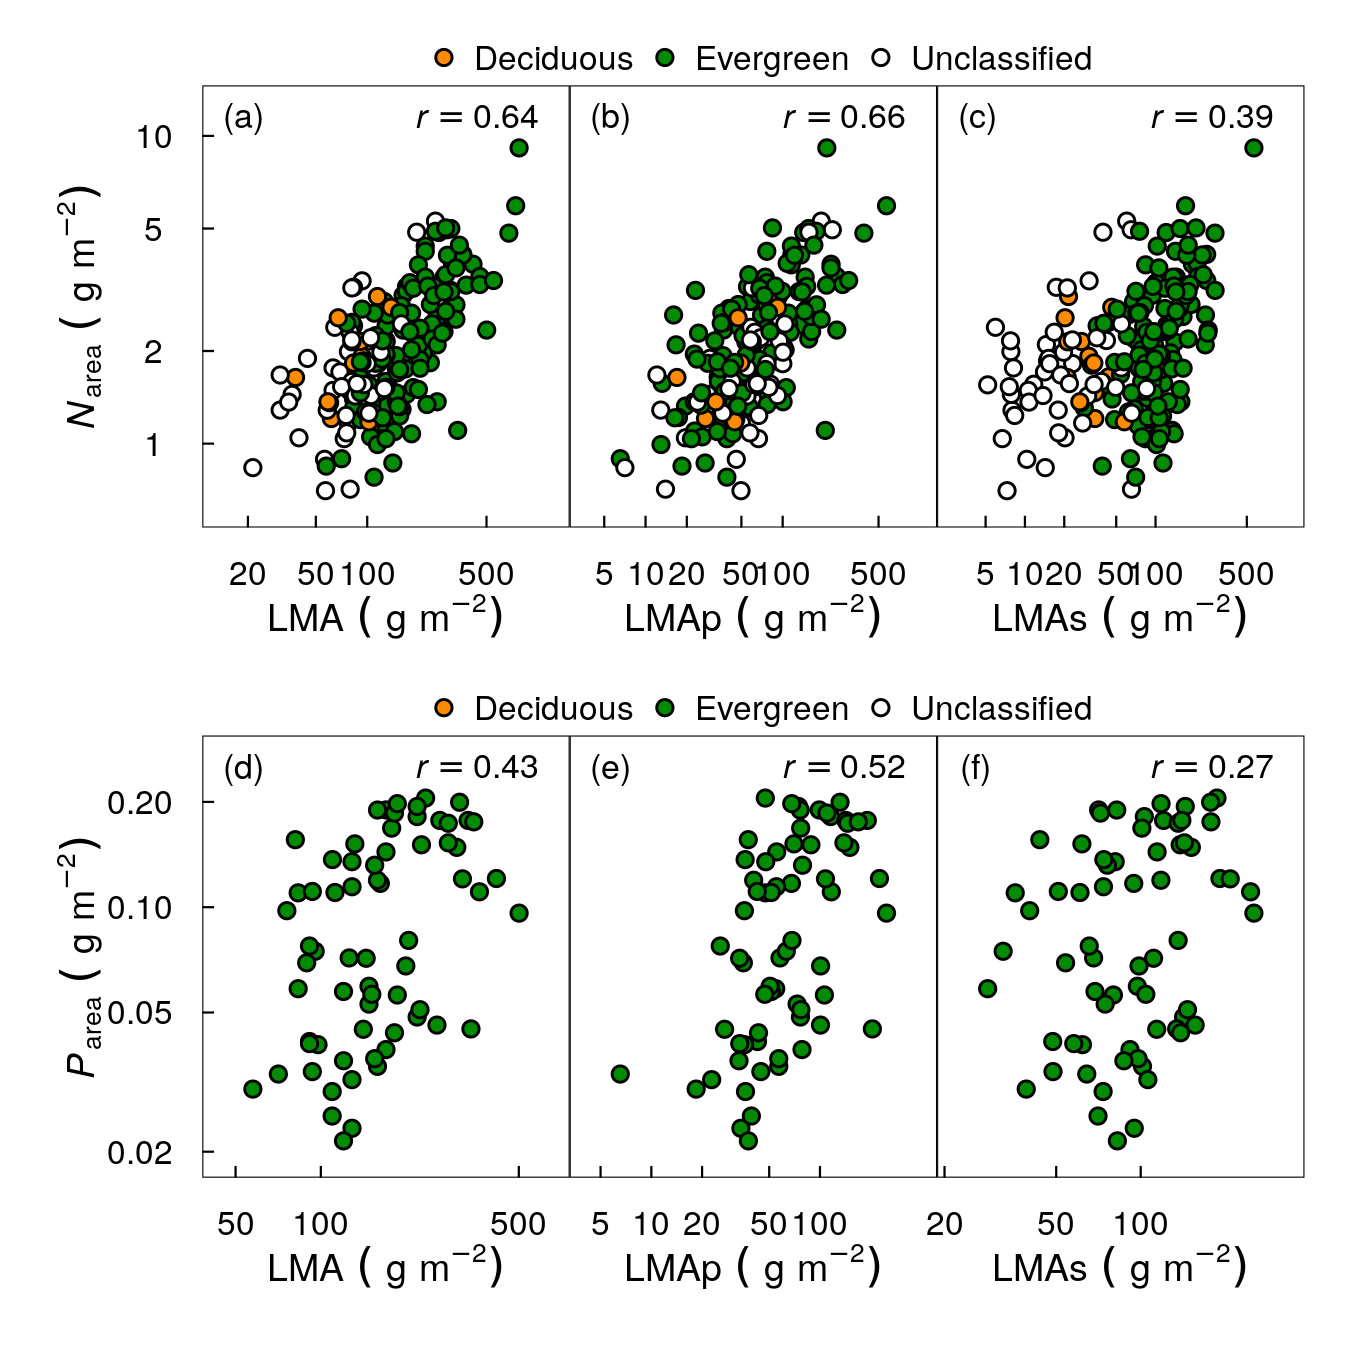
\includegraphics{/Users/mattocci/Dropbox/MS/LMAms/figs/gl_point_np2.png}

\textbf{Fig. S6}: Measured traits related to photosynthesis and
metabolism (nitrogen and phosphorus per-unit leaf area;
\emph{N}\textsubscript{area} and \emph{P}\textsubscript{area}) are
positively correlated with LMA and with estimates (posterior medians) of
the metabolic and structural LMA components (LMAm and LMAs,
respectively) in the GLOPNET dataset. LMAm yields more consistent
relationships compared to LMA and LMAs; e.g., evergreen and deciduous
leaves align along a single relationship in panel b, but not in panels a
or c.

\newpage

\hypertarget{fig.-s7}{%
\subsection{Fig. S7}\label{fig.-s7}}

\includegraphics{/Users/mattocci/Dropbox/MS/LMAms/figs/pa_point_npc_par.png}

\textbf{Fig. S7}: Partial regression plots for nitrogen, phosphorus and
cellulose per-unit leaf area (\emph{N}\textsubscript{area},
\emph{P}\textsubscript{area} and CL\textsubscript{area}). (a) LMAs
variation is controlled. (b) LMAm variation is controlled. The partial
regression plots show separation between sun and shade when controlling
for LMAs variation (i.e., LMAs does not explain the sun/shade
difference), but overlapping distributions of sun and shade when
controlling for LMAm variation (i.e., LMAm does explain the sun/shade
difference). Partial correlation coefficients (\(\rho\)) are shown.

\newpage

\hypertarget{fig.-s8}{%
\subsection{Fig. S8}\label{fig.-s8}}

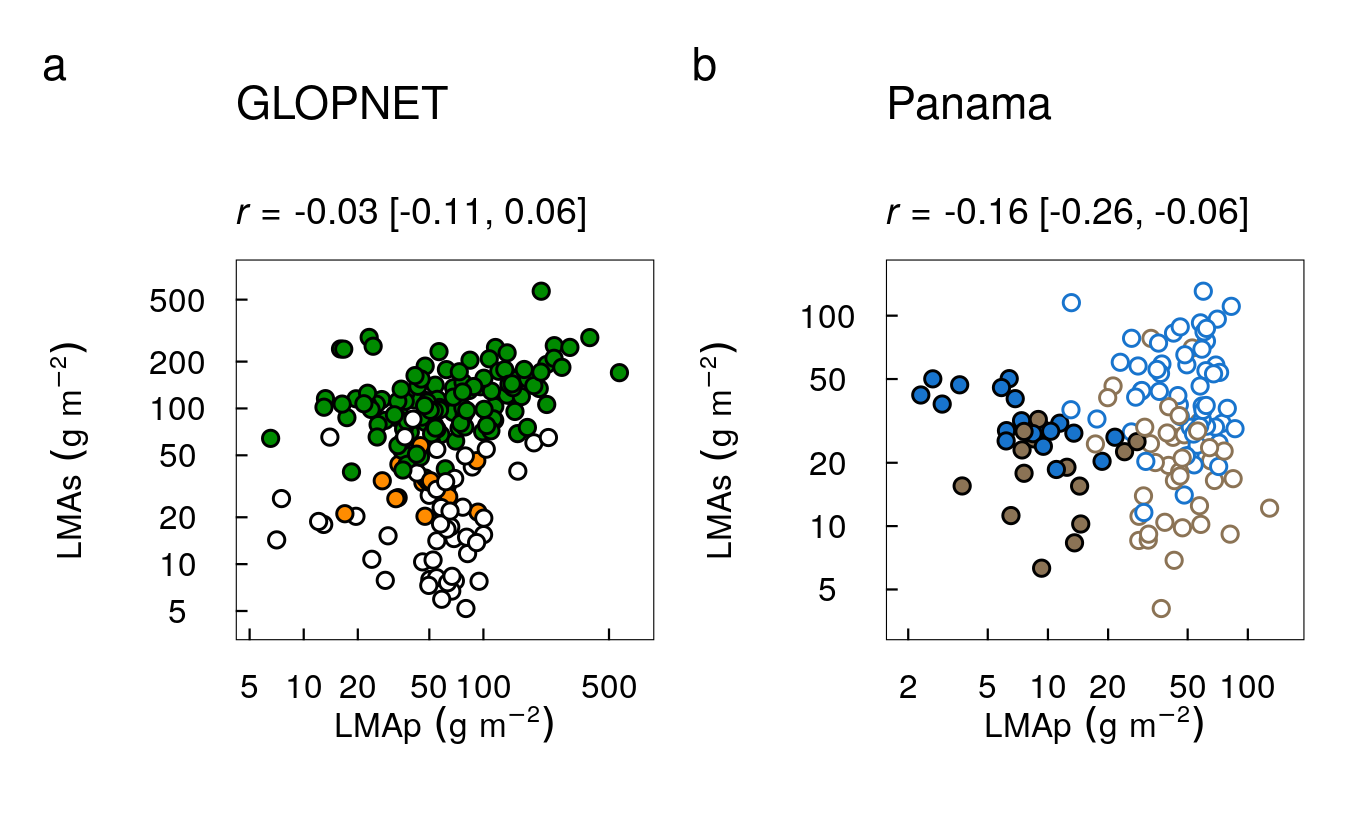
\includegraphics{/Users/mattocci/Dropbox/MS/LMAms/figs/ps_point.png}

\textbf{Fig. S8} Pearson correlation coefficients for posterior medians
of LMAm vs LMAs in the (a) GLOPNET and (b) Panama datasets. The
non-significant or weak \emph{r} values indicate that a single axis
could not accurately represent the two-dimensional space. Symbols as in
Main Text Figs. 2- 3.

\newpage

\hypertarget{appendix-s4-stan-code}{%
\section{Appendix S4: Stan code}\label{appendix-s4-stan-code}}

\hypertarget{stan-code-for-the-glopnet-dataset}{%
\subsection{Stan code for the GLOPNET
dataset}\label{stan-code-for-the-glopnet-dataset}}

The best model for the GLOPNET dataset is LMAm-LMAs with the constraint
of \(\beta_m\) = 0.

\begin{Shaded}
\begin{Highlighting}[]
\CommentTok{//}\AlertTok{NOTE}\CommentTok{: THIS STAN CODE IS GENERATED VIA "update.py"}
\KeywordTok{data}\NormalTok{ \{}
  \DataTypeTok{int}\NormalTok{\textless{}}\KeywordTok{lower}\NormalTok{=}\DecValTok{0}\NormalTok{\textgreater{} N;}
  \DataTypeTok{vector}\NormalTok{\textless{}}\KeywordTok{lower}\NormalTok{=}\DecValTok{0}\NormalTok{\textgreater{}[N] LMA;}
  \DataTypeTok{vector}\NormalTok{\textless{}}\KeywordTok{lower}\NormalTok{=}\DecValTok{0}\NormalTok{\textgreater{}[N] A;}
  \DataTypeTok{vector}\NormalTok{\textless{}}\KeywordTok{lower}\NormalTok{=}\DecValTok{0}\NormalTok{\textgreater{}[N] R;}
  \DataTypeTok{vector}\NormalTok{\textless{}}\KeywordTok{lower}\NormalTok{=}\DecValTok{0}\NormalTok{\textgreater{}[N] LL;}
\NormalTok{\}}

\KeywordTok{transformed data}\NormalTok{ \{}
  \DataTypeTok{vector}\NormalTok{[N] log\_A;}
  \DataTypeTok{vector}\NormalTok{[N] log\_LL;}
  \DataTypeTok{vector}\NormalTok{[N] log\_R;}
  \DataTypeTok{matrix}\NormalTok{[N, }\DecValTok{3}\NormalTok{] obs;}
  \DataTypeTok{vector}\NormalTok{[N] intercept;}
  \ControlFlowTok{for}\NormalTok{ (n }\ControlFlowTok{in} \DecValTok{1}\NormalTok{:N)}
\NormalTok{    intercept[n] = }\DecValTok{1}\NormalTok{;}
\NormalTok{  log\_A = log(A);}
\NormalTok{  log\_LL = log(LL);}
\NormalTok{  log\_R = log(R);}
  \CommentTok{// use net photosynthesis (A) instead of gross (A + R)}
\NormalTok{  obs = append\_col(append\_col(log\_A, log\_LL), log\_R);}
\NormalTok{\}}

\KeywordTok{parameters}\NormalTok{ \{}
  \DataTypeTok{real}\NormalTok{ a0;}
  \DataTypeTok{real}\NormalTok{ am;}
  \DataTypeTok{real}\NormalTok{ as;}
  \DataTypeTok{real}\NormalTok{ b0;}
  \DataTypeTok{real}\NormalTok{ bs;}
  \DataTypeTok{real}\NormalTok{ g0;}
  \DataTypeTok{real}\NormalTok{ gm;}
  \DataTypeTok{real}\NormalTok{ gs;}
  \DataTypeTok{vector}\NormalTok{\textless{}}\KeywordTok{lower}\NormalTok{=}\DecValTok{0}\NormalTok{, }\KeywordTok{upper}\NormalTok{=}\DecValTok{1}\NormalTok{\textgreater{}[N] p;}
  \DataTypeTok{vector}\NormalTok{\textless{}}\KeywordTok{lower}\NormalTok{=}\DecValTok{0}\NormalTok{\textgreater{}[}\DecValTok{3}\NormalTok{] L\_sigma;}
  \DataTypeTok{cholesky\_factor\_corr}\NormalTok{[}\DecValTok{3}\NormalTok{] L\_Omega;}
\NormalTok{\}}

\KeywordTok{transformed parameters}\NormalTok{ \{}
  \DataTypeTok{matrix}\NormalTok{[N, }\DecValTok{3}\NormalTok{] Mu;}
  \DataTypeTok{matrix}\NormalTok{[}\DecValTok{3}\NormalTok{, }\DecValTok{3}\NormalTok{] Z;}
  \DataTypeTok{matrix}\NormalTok{[N, }\DecValTok{3}\NormalTok{] X;}
\NormalTok{  Z[}\DecValTok{1}\NormalTok{, }\DecValTok{1}\NormalTok{] = a0;}
\NormalTok{  Z[}\DecValTok{1}\NormalTok{, }\DecValTok{2}\NormalTok{] = b0;}
\NormalTok{  Z[}\DecValTok{1}\NormalTok{, }\DecValTok{3}\NormalTok{] = g0;}
\NormalTok{  Z[}\DecValTok{2}\NormalTok{, }\DecValTok{1}\NormalTok{] = am;}
\NormalTok{  Z[}\DecValTok{2}\NormalTok{, }\DecValTok{2}\NormalTok{] = }\DecValTok{0}\NormalTok{;}
\NormalTok{  Z[}\DecValTok{2}\NormalTok{, }\DecValTok{3}\NormalTok{] = gm;}
\NormalTok{  Z[}\DecValTok{3}\NormalTok{, }\DecValTok{1}\NormalTok{] = as;}
\NormalTok{  Z[}\DecValTok{3}\NormalTok{, }\DecValTok{2}\NormalTok{] = bs;}
\NormalTok{  Z[}\DecValTok{3}\NormalTok{, }\DecValTok{3}\NormalTok{] = gs;}

  \CommentTok{//log\_LMAm = log(LMA) + log(p);}
  \CommentTok{//log\_LMAs = log(LMA) + log(1 {-} p);}
  \CommentTok{//X = append\_col(append\_col(append\_col(intercept, log\_LMAm), log\_LMAs), leaf);}
\NormalTok{  X = append\_col(append\_col(intercept, log(LMA) + log(p)), log(LMA) + log(}\DecValTok{1}\NormalTok{ {-} p));}
\NormalTok{  Mu = X * Z;}
\NormalTok{\}}

\KeywordTok{model}\NormalTok{ \{}
  \CommentTok{// priors}
\NormalTok{  a0 \textasciitilde{} normal(}\DecValTok{0}\NormalTok{, }\DecValTok{5}\NormalTok{);}
\NormalTok{  b0 \textasciitilde{} normal(}\DecValTok{0}\NormalTok{, }\DecValTok{5}\NormalTok{);}
\NormalTok{  g0 \textasciitilde{} normal(}\DecValTok{0}\NormalTok{, }\DecValTok{5}\NormalTok{);}
\NormalTok{  am \textasciitilde{} normal(}\DecValTok{0}\NormalTok{, }\DecValTok{5}\NormalTok{);}
\NormalTok{  bs \textasciitilde{} normal(}\DecValTok{0}\NormalTok{, }\DecValTok{5}\NormalTok{);}
\NormalTok{  gm \textasciitilde{} normal(}\DecValTok{0}\NormalTok{, }\DecValTok{5}\NormalTok{);}
\NormalTok{  gs \textasciitilde{} normal(}\DecValTok{0}\NormalTok{, }\DecValTok{5}\NormalTok{);}
\NormalTok{  as \textasciitilde{} normal(}\DecValTok{0}\NormalTok{, }\DecValTok{5}\NormalTok{);}
\NormalTok{  p \textasciitilde{} beta(}\DecValTok{1}\NormalTok{, }\DecValTok{1}\NormalTok{);}
\NormalTok{  L\_Omega \textasciitilde{} lkj\_corr\_cholesky(}\DecValTok{2}\NormalTok{);}
\NormalTok{  L\_sigma \textasciitilde{} cauchy(}\DecValTok{0}\NormalTok{, }\FloatTok{2.5}\NormalTok{);}

  \CommentTok{// model}
  \ControlFlowTok{for}\NormalTok{ (i }\ControlFlowTok{in} \DecValTok{1}\NormalTok{:N)}
     \KeywordTok{target +=}\NormalTok{ multi\_normal\_cholesky\_lpdf(obs[i,] | Mu[i,], diag\_pre\_multiply(L\_sigma, L\_Omega));}
\NormalTok{\}}

\KeywordTok{generated quantities}\NormalTok{ \{}
  \DataTypeTok{vector}\NormalTok{[N] log\_lik;}
  \DataTypeTok{real}\NormalTok{\textless{}}\KeywordTok{lower}\NormalTok{={-}}\DecValTok{1}\NormalTok{, }\KeywordTok{upper}\NormalTok{=}\DecValTok{1}\NormalTok{\textgreater{} rho12;}
  \DataTypeTok{real}\NormalTok{\textless{}}\KeywordTok{lower}\NormalTok{={-}}\DecValTok{1}\NormalTok{, }\KeywordTok{upper}\NormalTok{=}\DecValTok{1}\NormalTok{\textgreater{} rho23;}
  \DataTypeTok{real}\NormalTok{\textless{}}\KeywordTok{lower}\NormalTok{={-}}\DecValTok{1}\NormalTok{, }\KeywordTok{upper}\NormalTok{=}\DecValTok{1}\NormalTok{\textgreater{} rho13;}
  \DataTypeTok{cov\_matrix}\NormalTok{[}\DecValTok{3}\NormalTok{] Sigma;}
  \DataTypeTok{vector}\NormalTok{[N] log\_LMAm;}
  \DataTypeTok{vector}\NormalTok{[N] log\_LMAs;}
\NormalTok{  log\_LMAm = log(LMA) + log(p);}
\NormalTok{  log\_LMAs = log(LMA) + log(}\DecValTok{1}\NormalTok{ {-} p);}
\NormalTok{  Sigma = diag\_pre\_multiply(L\_sigma, L\_Omega)}
\NormalTok{     * diag\_post\_multiply(L\_Omega\textquotesingle{}, L\_sigma);}
\NormalTok{  rho12 = Sigma[}\DecValTok{1}\NormalTok{, }\DecValTok{2}\NormalTok{] * inv(L\_sigma[}\DecValTok{1}\NormalTok{] * L\_sigma[}\DecValTok{2}\NormalTok{]);}
\NormalTok{  rho23 = Sigma[}\DecValTok{2}\NormalTok{, }\DecValTok{3}\NormalTok{] * inv(L\_sigma[}\DecValTok{2}\NormalTok{] * L\_sigma[}\DecValTok{3}\NormalTok{]);}
\NormalTok{  rho13 = Sigma[}\DecValTok{1}\NormalTok{, }\DecValTok{3}\NormalTok{] * inv(L\_sigma[}\DecValTok{1}\NormalTok{] * L\_sigma[}\DecValTok{3}\NormalTok{]);}
  \ControlFlowTok{for}\NormalTok{ (i }\ControlFlowTok{in} \DecValTok{1}\NormalTok{:N)}
\NormalTok{   log\_lik[i] = multi\_normal\_cholesky\_lpdf(obs[i,] | Mu[i,], diag\_pre\_multiply(L\_sigma, L\_Omega));}
\NormalTok{ \}}
\end{Highlighting}
\end{Shaded}

\hypertarget{stan-code-for-the-panama-dataset}{%
\subsection{Stan code for the Panama
dataset}\label{stan-code-for-the-panama-dataset}}

The best model for the Panama dataset is LMAm-LMAs-light with the
constraint of \(\alpha_s\) = 0 and \(\beta_m\) = 0.

\begin{Shaded}
\begin{Highlighting}[]
\CommentTok{//}\AlertTok{NOTE}\CommentTok{: THIS STAN CODE IS GENERATED VIA "update.py"}
\KeywordTok{data}\NormalTok{ \{}
  \DataTypeTok{int}\NormalTok{\textless{}}\KeywordTok{lower}\NormalTok{=}\DecValTok{0}\NormalTok{\textgreater{} N;}
  \DataTypeTok{vector}\NormalTok{\textless{}}\KeywordTok{lower}\NormalTok{=}\DecValTok{0}\NormalTok{\textgreater{}[N] LMA;}
  \DataTypeTok{vector}\NormalTok{\textless{}}\KeywordTok{lower}\NormalTok{=}\DecValTok{0}\NormalTok{\textgreater{}[N] A;}
  \DataTypeTok{vector}\NormalTok{\textless{}}\KeywordTok{lower}\NormalTok{=}\DecValTok{0}\NormalTok{\textgreater{}[N] R;}
  \DataTypeTok{vector}\NormalTok{\textless{}}\KeywordTok{lower}\NormalTok{=}\DecValTok{0}\NormalTok{\textgreater{}[N] LL;}
  \DataTypeTok{vector}\NormalTok{\textless{}}\KeywordTok{lower}\NormalTok{=}\DecValTok{0}\NormalTok{\textgreater{}[N] leaf;}
\NormalTok{\}}

\KeywordTok{transformed data}\NormalTok{ \{}
  \DataTypeTok{vector}\NormalTok{[N] log\_A;}
  \DataTypeTok{vector}\NormalTok{[N] log\_LL;}
  \DataTypeTok{vector}\NormalTok{[N] log\_R;}
  \DataTypeTok{matrix}\NormalTok{[N, }\DecValTok{3}\NormalTok{] obs;}
  \DataTypeTok{vector}\NormalTok{[N] intercept;}
  \ControlFlowTok{for}\NormalTok{ (n }\ControlFlowTok{in} \DecValTok{1}\NormalTok{:N)}
\NormalTok{    intercept[n] = }\DecValTok{1}\NormalTok{;}
\NormalTok{  log\_A = log(A);}
\NormalTok{  log\_LL = log(LL);}
\NormalTok{  log\_R = log(R);}
  \CommentTok{// use net photosynthesis (A) instead of gross (A + R)}
\NormalTok{  obs = append\_col(append\_col(log\_A, log\_LL), log\_R);}
\NormalTok{\}}

\KeywordTok{parameters}\NormalTok{ \{}
  \DataTypeTok{real}\NormalTok{ a0;}
  \DataTypeTok{real}\NormalTok{ am;}
  \DataTypeTok{real}\NormalTok{ b0;}
  \DataTypeTok{real}\NormalTok{ bs;}
  \DataTypeTok{real}\NormalTok{ g0;}
  \DataTypeTok{real}\NormalTok{ gm;}
  \DataTypeTok{real}\NormalTok{ gs;}
  \DataTypeTok{real}\NormalTok{ theta;}
  \DataTypeTok{vector}\NormalTok{\textless{}}\KeywordTok{lower}\NormalTok{=}\DecValTok{0}\NormalTok{, }\KeywordTok{upper}\NormalTok{=}\DecValTok{1}\NormalTok{\textgreater{}[N] p;}
  \DataTypeTok{vector}\NormalTok{\textless{}}\KeywordTok{lower}\NormalTok{=}\DecValTok{0}\NormalTok{\textgreater{}[}\DecValTok{3}\NormalTok{] L\_sigma;}
  \DataTypeTok{cholesky\_factor\_corr}\NormalTok{[}\DecValTok{3}\NormalTok{] L\_Omega;}
\NormalTok{\}}

\KeywordTok{transformed parameters}\NormalTok{ \{}
  \DataTypeTok{matrix}\NormalTok{[N, }\DecValTok{3}\NormalTok{] Mu;}
  \DataTypeTok{matrix}\NormalTok{[}\DecValTok{4}\NormalTok{, }\DecValTok{3}\NormalTok{] Z;}
  \DataTypeTok{matrix}\NormalTok{[N, }\DecValTok{4}\NormalTok{] X;}
\NormalTok{  Z[}\DecValTok{1}\NormalTok{, }\DecValTok{1}\NormalTok{] = a0;}
\NormalTok{  Z[}\DecValTok{1}\NormalTok{, }\DecValTok{2}\NormalTok{] = b0;}
\NormalTok{  Z[}\DecValTok{1}\NormalTok{, }\DecValTok{3}\NormalTok{] = g0;}
\NormalTok{  Z[}\DecValTok{2}\NormalTok{, }\DecValTok{1}\NormalTok{] = am;}
\NormalTok{  Z[}\DecValTok{2}\NormalTok{, }\DecValTok{2}\NormalTok{] = }\DecValTok{0}\NormalTok{;}
\NormalTok{  Z[}\DecValTok{2}\NormalTok{, }\DecValTok{3}\NormalTok{] = gm;}
\NormalTok{  Z[}\DecValTok{3}\NormalTok{, }\DecValTok{1}\NormalTok{] = }\DecValTok{0}\NormalTok{;}
\NormalTok{  Z[}\DecValTok{3}\NormalTok{, }\DecValTok{2}\NormalTok{] = bs;}
\NormalTok{  Z[}\DecValTok{3}\NormalTok{, }\DecValTok{3}\NormalTok{] = gs;}
\NormalTok{  Z[}\DecValTok{4}\NormalTok{, }\DecValTok{1}\NormalTok{] = }\DecValTok{0}\NormalTok{;}
\NormalTok{  Z[}\DecValTok{4}\NormalTok{, }\DecValTok{2}\NormalTok{] = theta;}
\NormalTok{  Z[}\DecValTok{4}\NormalTok{, }\DecValTok{3}\NormalTok{] = }\DecValTok{0}\NormalTok{;}

  \CommentTok{//log\_LMAm = log(LMA) + log(p);}
  \CommentTok{//log\_LMAs = log(LMA) + log(1 {-} p);}
  \CommentTok{//X = append\_col(append\_col(append\_col(intercept, log\_LMAm), log\_LMAs), leaf);}
\NormalTok{  X = append\_col(append\_col(append\_col(intercept,}
\NormalTok{    log(LMA) + log(p)),}
\NormalTok{    log(LMA) + log(}\DecValTok{1}\NormalTok{ {-} p)),}
\NormalTok{    leaf);}
\NormalTok{  Mu = X * Z;}
\NormalTok{\}}

\KeywordTok{model}\NormalTok{ \{}
  \CommentTok{// priors}
\NormalTok{  a0 \textasciitilde{} normal(}\DecValTok{0}\NormalTok{, }\DecValTok{5}\NormalTok{);}
\NormalTok{  b0 \textasciitilde{} normal(}\DecValTok{0}\NormalTok{, }\DecValTok{5}\NormalTok{);}
\NormalTok{  g0 \textasciitilde{} normal(}\DecValTok{0}\NormalTok{, }\DecValTok{5}\NormalTok{);}
\NormalTok{  am \textasciitilde{} normal(}\DecValTok{0}\NormalTok{, }\DecValTok{5}\NormalTok{);}
\NormalTok{  bs \textasciitilde{} normal(}\DecValTok{0}\NormalTok{, }\DecValTok{5}\NormalTok{);}
\NormalTok{  gm \textasciitilde{} normal(}\DecValTok{0}\NormalTok{, }\DecValTok{5}\NormalTok{);}
\NormalTok{  gs \textasciitilde{} normal(}\DecValTok{0}\NormalTok{, }\DecValTok{5}\NormalTok{);}
\NormalTok{  theta \textasciitilde{} normal(}\DecValTok{0}\NormalTok{, }\DecValTok{5}\NormalTok{);}
\NormalTok{  p \textasciitilde{} beta(}\DecValTok{1}\NormalTok{, }\DecValTok{1}\NormalTok{);}
\NormalTok{  L\_Omega \textasciitilde{} lkj\_corr\_cholesky(}\DecValTok{2}\NormalTok{);}
\NormalTok{  L\_sigma \textasciitilde{} cauchy(}\DecValTok{0}\NormalTok{, }\FloatTok{2.5}\NormalTok{);}

  \CommentTok{// model}
  \ControlFlowTok{for}\NormalTok{ (i }\ControlFlowTok{in} \DecValTok{1}\NormalTok{:N)}
     \KeywordTok{target +=}\NormalTok{ multi\_normal\_cholesky\_lpdf(obs[i,] | Mu[i,], diag\_pre\_multiply(L\_sigma, L\_Omega));}
\NormalTok{\}}

\KeywordTok{generated quantities}\NormalTok{ \{}
  \DataTypeTok{vector}\NormalTok{[N] log\_lik;}
  \DataTypeTok{real}\NormalTok{\textless{}}\KeywordTok{lower}\NormalTok{={-}}\DecValTok{1}\NormalTok{, }\KeywordTok{upper}\NormalTok{=}\DecValTok{1}\NormalTok{\textgreater{} rho12;}
  \DataTypeTok{real}\NormalTok{\textless{}}\KeywordTok{lower}\NormalTok{={-}}\DecValTok{1}\NormalTok{, }\KeywordTok{upper}\NormalTok{=}\DecValTok{1}\NormalTok{\textgreater{} rho23;}
  \DataTypeTok{real}\NormalTok{\textless{}}\KeywordTok{lower}\NormalTok{={-}}\DecValTok{1}\NormalTok{, }\KeywordTok{upper}\NormalTok{=}\DecValTok{1}\NormalTok{\textgreater{} rho13;}
  \DataTypeTok{cov\_matrix}\NormalTok{[}\DecValTok{3}\NormalTok{] Sigma;}
  \DataTypeTok{vector}\NormalTok{[N] log\_LMAm;}
  \DataTypeTok{vector}\NormalTok{[N] log\_LMAs;}
\NormalTok{  log\_LMAm = log(LMA) + log(p);}
\NormalTok{  log\_LMAs = log(LMA) + log(}\DecValTok{1}\NormalTok{ {-} p);}
\NormalTok{  Sigma = diag\_pre\_multiply(L\_sigma, L\_Omega)}
\NormalTok{     * diag\_post\_multiply(L\_Omega\textquotesingle{}, L\_sigma);}
\NormalTok{  rho12 = Sigma[}\DecValTok{1}\NormalTok{, }\DecValTok{2}\NormalTok{] * inv(L\_sigma[}\DecValTok{1}\NormalTok{] * L\_sigma[}\DecValTok{2}\NormalTok{]);}
\NormalTok{  rho23 = Sigma[}\DecValTok{2}\NormalTok{, }\DecValTok{3}\NormalTok{] * inv(L\_sigma[}\DecValTok{2}\NormalTok{] * L\_sigma[}\DecValTok{3}\NormalTok{]);}
\NormalTok{  rho13 = Sigma[}\DecValTok{1}\NormalTok{, }\DecValTok{3}\NormalTok{] * inv(L\_sigma[}\DecValTok{1}\NormalTok{] * L\_sigma[}\DecValTok{3}\NormalTok{]);}
  \ControlFlowTok{for}\NormalTok{ (i }\ControlFlowTok{in} \DecValTok{1}\NormalTok{:N)}
\NormalTok{   log\_lik[i] = multi\_normal\_cholesky\_lpdf(obs[i,] | Mu[i,], diag\_pre\_multiply(L\_sigma, L\_Omega));}
\NormalTok{ \}}
\end{Highlighting}
\end{Shaded}

\hypertarget{references}{%
\section*{References}\label{references}}
\addcontentsline{toc}{section}{References}

\hypertarget{refs}{}
\begin{CSLReferences}{1}{0}
\leavevmode\vadjust pre{\hypertarget{ref-Alvarez2014}{}}%
Alvarez, I., Niemi, J., \& Simpson, M. (2014). Bayesian inference for a
covariance matrix. \emph{arXiv Preprint arXiv:1408.4050v2}, 1--12.
\url{https://doi.org/10.1214/aos/1176348885}

\leavevmode\vadjust pre{\hypertarget{ref-Gelman2008}{}}%
Gelman, A., Jakulin, A., Pittau, M. G., \& Su, Y. S. (2008). A weakly
informative default prior distribution for logistic and other regression
models. \emph{Annals of Applied Statistics}, \emph{2}(4), 1360--1383.
\url{https://doi.org/10.1214/08-AOAS191}

\leavevmode\vadjust pre{\hypertarget{ref-Lemoine2019}{}}%
Lemoine, N. P. (2019). Moving beyond noninformative priors: Why and how
to choose weakly informative priors in {Bayesian} analyses.
\emph{Oikos}, \emph{128}(7), 912--928.
\url{https://doi.org/10.1111/oik.05985}

\leavevmode\vadjust pre{\hypertarget{ref-Lewandowski2009}{}}%
Lewandowski, D., Kurowicka, D., \& Joe, H. (2009). Generating random
correlation matrices based on vines and extended onion method.
\emph{Journal of Multivariate Analysis}, \emph{100}(9), 1989--2001.
\url{https://doi.org/10.1016/j.jmva.2009.04.008}

\leavevmode\vadjust pre{\hypertarget{ref-Osnas2018}{}}%
Osnas, J. L. D., Katabuchi, M., Kitajima, K., Wright, S. J., Reich, P.
B., Van Bael, S. A., \ldots{} Lichstein, J. W. (2018). Divergent drivers
of leaf trait variation within species, among species, and among
functional groups. \emph{Proceedings of the National Academy of Sciences
of the United States of America}, \emph{115}(21), 5480--5485.
\url{https://doi.org/10.1073/pnas.1803989115}

\end{CSLReferences}



\end{document}
